\documentclass{ximera}


\graphicspath{
  {./}
  {ximeraTutorial/}
  {basicPhilosophy/}
}

\newcommand{\mooculus}{\textsf{\textbf{MOOC}\textnormal{\textsf{ULUS}}}}

\usepackage{tkz-euclide}\usepackage{tikz}
\usepackage{tikz-cd}
\usetikzlibrary{arrows}
\tikzset{>=stealth,commutative diagrams/.cd,
  arrow style=tikz,diagrams={>=stealth}} %% cool arrow head
\tikzset{shorten <>/.style={ shorten >=#1, shorten <=#1 } } %% allows shorter vectors

\usetikzlibrary{backgrounds} %% for boxes around graphs
\usetikzlibrary{shapes,positioning}  %% Clouds and stars
\usetikzlibrary{matrix} %% for matrix
\usepgfplotslibrary{polar} %% for polar plots
\usepgfplotslibrary{fillbetween} %% to shade area between curves in TikZ
\usetkzobj{all}
\usepackage[makeroom]{cancel} %% for strike outs
%\usepackage{mathtools} %% for pretty underbrace % Breaks Ximera
%\usepackage{multicol}
\usepackage{pgffor} %% required for integral for loops



%% http://tex.stackexchange.com/questions/66490/drawing-a-tikz-arc-specifying-the-center
%% Draws beach ball
\tikzset{pics/carc/.style args={#1:#2:#3}{code={\draw[pic actions] (#1:#3) arc(#1:#2:#3);}}}



\usepackage{array}
\setlength{\extrarowheight}{+.1cm}
\newdimen\digitwidth
\settowidth\digitwidth{9}
\def\divrule#1#2{
\noalign{\moveright#1\digitwidth
\vbox{\hrule width#2\digitwidth}}}






\DeclareMathOperator{\arccot}{arccot}
\DeclareMathOperator{\arcsec}{arcsec}
\DeclareMathOperator{\arccsc}{arccsc}

















%%This is to help with formatting on future title pages.
\newenvironment{sectionOutcomes}{}{}


\author{Lee Wayand}

\begin{document}
\begin{exercise}  





Below is the graph of $y=f(x)$.  

\begin{image}
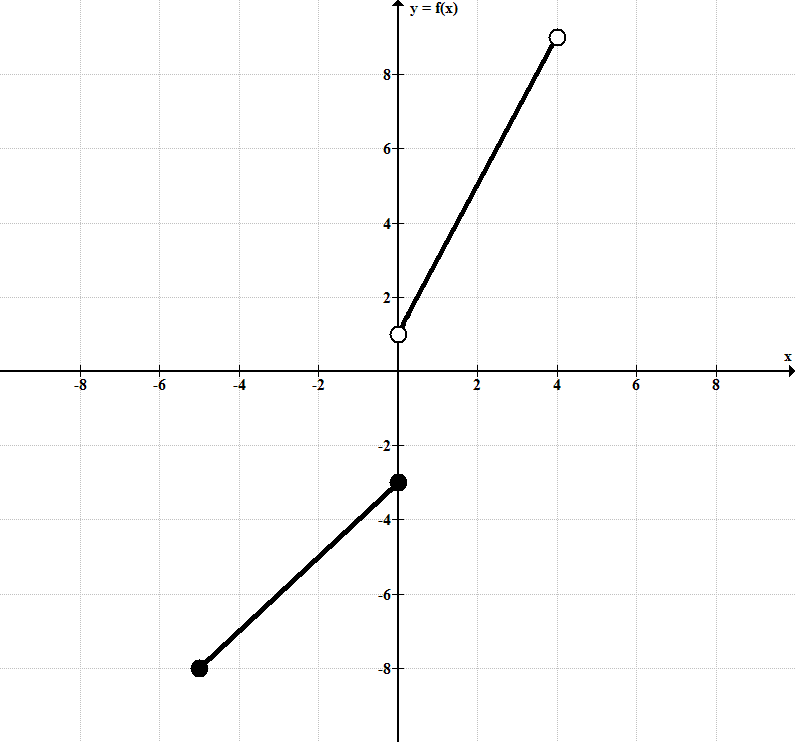
\includegraphics{../../pics/func_graphs/f29.png}
\end{image}


\begin{question} 

What is the domain of $f$?


\begin{multipleChoice}
\choice {$[-5, 0) \cup (0, 4)$}
\choice [correct]{$[-5, 4)$}
\choice {$(-\infty, \infty)$}
\choice {$(-\infty, 0) \cup (0, \infty)$}
\choice {$[-8, -3] \cup (1, 9)$}
\end{multipleChoice}

\end{question}





\begin{question} 


Evaluate $f(0) = \answer[tolerance=0.25]{-3}$


Classify $0$. \\


\begin{multipleChoice}
\choice [correct]{Discontinuity}
\choice {Singularity}
\choice {Neither}
\end{multipleChoice}



\end{question}










\begin{question} 


$f$ is increasing on $(-5, 0)$. \\


\begin{multipleChoice}
\choice [correct]{True}
\choice {False}
\end{multipleChoice}




$f$ is increasing on $[-5, 0]$. \\


\begin{multipleChoice}
\choice [correct]{True}
\choice {False}
\end{multipleChoice}





$f$ is increasing on $(-5, 0]$. \\


\begin{multipleChoice}
\choice [correct]{True}
\choice {False}
\end{multipleChoice}




$f$ is increasing on $[-5, 0)$. \\


\begin{multipleChoice}
\choice [correct]{True}
\choice {False}
\end{multipleChoice}



\end{question}















\begin{question} 


$f$ is increasing on $(0, 4)$. \\


\begin{multipleChoice}
\choice [correct]{True}
\choice {False}
\end{multipleChoice}




$f$ is increasing on $[0, 4]$. \\


\begin{multipleChoice}
\choice {True}
\choice [correct]{False}
\end{multipleChoice}





$f$ is increasing on $[0, 4)$. \\


\begin{multipleChoice}
\choice [correct]{True}
\choice {False}
\end{multipleChoice}



\end{question}







\begin{question} 

There exists a real number, $M$, such that $f(x) < M$ for all $k$.
\begin{multipleChoice}
\choice [correct]{True}
\choice {False}
\end{multipleChoice}

\end{question}





\begin{question} 

There exists a real number, $M$, such that $f(k) > M$ for all $k$.
\begin{multipleChoice}
\choice [correct]{True}
\choice {False}
\end{multipleChoice}

\end{question}








\begin{question} 

For any $\epsilon > 0$, there exists a domain number in the interval $(0-\epsilon, 0+\epsilon)$.
\begin{multipleChoice}
\choice [correct]{True}
\choice {False}
\end{multipleChoice}


\end{question}







\begin{question} 

For any $\epsilon > 0$, there exists a domain number in the interval $(-5-\epsilon, -5+\epsilon)$.
\begin{multipleChoice}
\choice [correct]{True}
\choice {False}
\end{multipleChoice}


\end{question}








\begin{question} 

For any $\epsilon > 0$, there exists a domain number, $d$, in the interval $(0-\epsilon, 0+\epsilon)$ such that $f(d) - f(0) > 1$.
\begin{multipleChoice}
\choice [correct]{True}
\choice {False}
\end{multipleChoice}


\end{question}










\begin{question} 

There exists an open interval, $I$, such that $2 < f(c) < 6$ for all $c \in I$.
\begin{multipleChoice}
\choice [correct]{True}
\choice {False}
\end{multipleChoice}


\end{question}











\begin{question} 

There exists a domain number, $c$, such that $f(c) < -9$.
\begin{multipleChoice}
\choice {True}
\choice [correct]{False}
\end{multipleChoice}


\end{question}












\begin{question} 

How many zeros does $f$ have?
\begin{multipleChoice}
\choice [correct] {$0$}
\choice {$1$}
\choice {$2$}
\choice {$3$}
\choice {$4$}
\end{multipleChoice}


\end{question}






\begin{question} 

$f$ is an increasing function.
\begin{multipleChoice}
\choice [correct]{True}
\choice {False}
\end{multipleChoice}


\end{question}







\begin{question} 

$f$ is continuous on the interval $(1, 3)$.
\begin{multipleChoice}
\choice [correct]{True}
\choice {False}
\end{multipleChoice}


\end{question}






\end{exercise}
\end{document}